\documentclass[16pt]{article}
\usepackage[utf8]{inputenc, lscape}
\usepackage[demo]{graphicx}
\usepackage[a4paper,bindingoffset=0.2in,%
            left=1.1in,right=0.85in,top=1in,bottom=1in,%
            footskip=.25in]{geometry}

\begin{document}

% data is from the presentation "cis_prel_pres" 3 days ago (levels) and 
% the scripts "i6_d25_6m_", "i6_d24_csd".

\newgeometry{left=1.5cm, right=1cm, top=3cm, bottom=1.5cm}

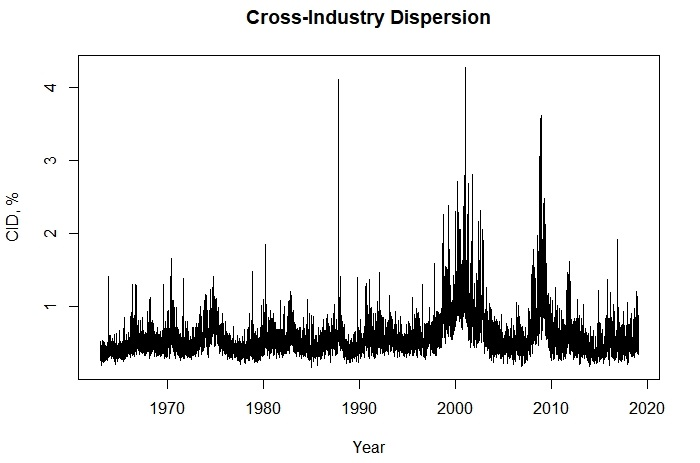
\includegraphics[width=1\textwidth]{ts_cid_00.jpeg}

\newpage

\textbf{Results with daily returns:}


% Table created by stargazer v.5.2.2 by Marek Hlavac, Harvard University. E-mail: hlavac at fas.harvard.edu
% Date and time: Wed, Aug 28, 2019 - 9:54:29 PM
\begin{table}[!htbp] \centering 
  \caption{Annualized excess returns of $\beta_{CID}$-sorted decile portfolios} 
  \label{} 
\begin{tabular}{@{\extracolsep{5pt}} cccccccccccc} 
\\[-1.8ex]\hline 
\hline \\[-1.8ex] 
 & D1 & D2 & D3 & D4 & D5 & D6 & D7 & D8 & D9 & D10 & LS \\ 
\hline \\[-1.8ex] 
Mean ew & $18.54$ & $15.45$ & $14.00$ & $13.11$ & $12.54$ & $12.55$ & $11.77$ & $11.51$ & $11.02$ & $12.24$ & $$-$6.27$ \\ 
T-stat & $8.12$ & $8.08$ & $7.78$ & $7.40$ & $7.06$ & $6.87$ & $6.25$ & $5.81$ & $5.15$ & $4.68$ & $$-$3.62$ \\ 
Mean vw & $12.15$ & $10.04$ & $7.88$ & $8.15$ & $8.19$ & $7.43$ & $6.56$ & $5.97$ & $4.33$ & $3.95$ & $$-$8.16$ \\ 
T-stat & $4.65$ & $4.56$ & $3.82$ & $4.01$ & $4.05$ & $3.62$ & $3.11$ & $2.72$ & $1.83$ & $1.36$ & $$-$3.57$ \\ 
\hline \\[-1.8ex] 
\end{tabular} 
\end{table}


% Table created by stargazer v.5.2.2 by Marek Hlavac, Harvard University. E-mail: hlavac at fas.harvard.edu
% Date and time: Wed, Aug 28, 2019 - 9:55:41 PM
\begin{table}[!htbp] \centering 
  \caption{Abnormal returns of vw L/S portfolios from decile sorts on $\beta_{CID}$} 
  \label{} 
\begin{tabular}{@{\extracolsep{5pt}} cccccc} 
\\[-1.8ex]\hline 
\hline \\[-1.8ex] 
Statistic & Ret & Alpha CAPM & Alpha FF3 & Alpha FF5 & Alpha FF5+UMD+LIQ \\ 
\hline \\[-1.8ex] 
LS & -8.139 & -9.223 & -10.810 & -9.727 & -5.569 \\ 
 & [ -3.57] & [ -4.08] & [ -5.00] & [ -4.50] & [ -2.66] \\ 
\hline \\[-1.8ex] 
\end{tabular} 
\end{table}


% Table created by stargazer v.5.2.2 by Marek Hlavac, Harvard University. E-mail: hlavac at fas.harvard.edu
% Date and time: Wed, Aug 28, 2019 - 9:57:16 PM
\begin{table}[!htbp] \centering 
  \caption{Loadings} 
  \label{} 
\begin{tabular}{@{\extracolsep{5pt}} ccccccccc} 
\\[-1.8ex]\hline 
\hline \\[-1.8ex] 
Ntile & Ret & Alpha & EMKT & HML & SMB & RMW & CMA & adjR2 \\ 
\hline \\[-1.8ex] 
1 & 12.096 & 6.5016 & 1.0417 & -0.2035 & 0.3362 & -0.0881 & -0.1318 & 0.7582 \\ 
 & [ 4.6342] & [ 5.0479] & [ 177.5799] & [ -16.4856] & [ 31.4218] & [ -5.8185] & [ -7.4064] &  \\ 
2 & 9.9792 & 3.4524 & 0.9634 & -0.0933 & 0.1845 & 0.0955 & 0.0735 & 0.8173 \\ 
 & [ 4.5356] & [ 3.6674] & [ 225.7348] & [ -10.3316] & [ 23.6501] & [ 8.6185] & [ 5.6414] &  \\ 
3 & 7.8372 & 1.4364 & 0.9228 & -0.0730 & 0.1206 & 0.1064 & 0.1086 & 0.8406 \\ 
 & [ 3.7988] & [ 1.7358] & [ 246.9307] & [ -9.2272] & [ 17.6417] & [ 10.9562] & [ 9.5108] &  \\ 
4 & 8.0892 & 1.6632 & 0.9246 & -0.0574 & 0.0578 & 0.1029 & 0.1415 & 0.8664 \\ 
 & [ 3.9879] & [ 2.2198] & [ 274.8004] & [ -8.0613] & [ 9.3881] & [ 11.7668] & [ 13.7711] &  \\ 
5 & 8.1648 & 1.4364 & 0.9326 & 0.0049 & 0.0036 & 0.1240 & 0.1367 & 0.8826 \\ 
 & [ 4.0324] & [ 2.0836] & [ 297.0358] & [ 0.7400] & [ 0.6434] & [ 15.1965] & [ 14.2570] &  \\ 
6 & 7.3836 & 0.4032 & 0.9561 & 0.0375 & -0.0028 & 0.1285 & 0.1376 & 0.8947 \\ 
 & [ 3.5969] & [ 0.5935] & [ 316.5355] & [ 5.8709] & [ -0.5147] & [ 16.3794] & [ 14.9250] &  \\ 
7 & 6.5268 & -0.6048 & 0.9794 & 0.0510 & -0.0216 & 0.1353 & 0.1261 & 0.8934 \\ 
 & [ 3.0969] & [ -0.8730] & [ 313.8990] & [ 7.7220] & [ -3.8400] & [ 16.6932] & [ 13.2421] &  \\ 
8 & 5.922 & -1.386 & 1.0109 & 0.1116 & -0.0248 & 0.1440 & 0.0356 & 0.8908 \\ 
 & [ 2.6934] & [ -1.8929] & [ 307.5378] & [ 16.0428] & [ -4.1833] & [ 16.8599] & [ 3.5465] &  \\ 
9 & 4.284 & -3.276 & 1.0772 & 0.1929 & -0.0442 & 0.0829 & -0.0302 & 0.8815 \\ 
 & [ 1.8100] & [ -4.0032] & [ 291.1920] & [ 24.6455] & [ -6.6266] & [ 8.6223] & [ -2.6715] &  \\ 
10 & 3.906 & -3.2256 & 1.2022 & 0.4106 & -0.0306 & -0.1627 & -0.4185 & 0.8158 \\ 
 & [ 1.3490] & [ -2.5902] & [ 213.5576] & [ 34.4841] & [ -3.0186] & [ -11.1194] & [ -24.3469] &  \\ 
LS & -8.1396 & -9.7272 & 0.1729 & 0.6257 & -0.3767 & -0.0811 & -0.2752 & 0.1129 \\ 
 & [ -3.5727] & [ -4.5071] & [ 17.6182] & [ 30.2858] & [ -21.0409] & [ -3.2020] & [ -9.2440] &  \\ 
\hline \\[-1.8ex] 
\end{tabular} 
\end{table}


% Table created by stargazer v.5.2.2 by Marek Hlavac, Harvard University. E-mail: hlavac at fas.harvard.edu
% Date and time: Wed, Aug 28, 2019 - 9:58:48 PM
\begin{table}[!htbp] \centering 
  \caption{Characteristics of decile $\beta_{CID}$-sorted portfolios} 
  \label{} 
\begin{tabular}{@{\extracolsep{5pt}} cccccccccccc} 
\\[-1.8ex]\hline 
\hline \\[-1.8ex] 
 & D1 & D2 & D3 & D4 & D5 & D6 & D7 & D8 & D9 & D10 & LS \\ 
\hline \\[-1.8ex] 
RET & $12.15$ & $10.04$ & $7.88$ & $8.15$ & $8.19$ & $7.43$ & $6.56$ & $5.97$ & $4.33$ & $3.95$ & $$-$8.16$ \\ 
T-stat & $4.65$ & $4.56$ & $3.82$ & $4.01$ & $4.05$ & $3.62$ & $3.11$ & $2.72$ & $1.83$ & $1.36$ & $$-$3.57$ \\ 
size & $14.48$ & $15.06$ & $15.32$ & $15.52$ & $15.66$ & $15.78$ & $15.87$ & $15.91$ & $15.85$ & $15.45$ & $0.96$ \\ 
bm & $$-$1.00$ & $$-$0.91$ & $$-$0.89$ & $$-$0.88$ & $$-$0.87$ & $$-$0.87$ & $$-$0.89$ & $$-$0.94$ & $$-$0.96$ & $$-$0.99$ & $0.01$ \\ 
op & $0.16$ & $0.17$ & $0.17$ & $0.17$ & $0.17$ & $0.17$ & $0.18$ & $0.18$ & $0.18$ & $0.17$ & $0.01$ \\ 
inv & $0.24$ & $0.18$ & $0.15$ & $0.14$ & $0.14$ & $0.13$ & $0.14$ & $0.14$ & $0.15$ & $0.20$ & $$-$0.05$ \\ 
beta & $1.01$ & $0.92$ & $0.90$ & $0.90$ & $0.91$ & $0.92$ & $0.95$ & $1.01$ & $1.08$ & $1.24$ & $0.23$ \\ 
BAspr & $0.33$ & $0.25$ & $0.22$ & $0.21$ & $0.20$ & $0.19$ & $0.19$ & $0.18$ & $0.19$ & $0.21$ & $$-$0.12$ \\ 
mom122 & $21.17$ & $15.43$ & $13.56$ & $12.94$ & $12.15$ & $11.80$ & $11.53$ & $11.53$ & $12.10$ & $13.89$ & $$-$7.28$ \\ 
vol1m & $2.24$ & $1.80$ & $1.66$ & $1.60$ & $1.57$ & $1.56$ & $1.58$ & $1.64$ & $1.76$ & $2.16$ & $$-$0.08$ \\ 
vol12m & $2.23$ & $1.84$ & $1.72$ & $1.66$ & $1.64$ & $1.63$ & $1.65$ & $1.71$ & $1.83$ & $2.20$ & $$-$0.02$ \\ 
\hline \\[-1.8ex] 
\end{tabular} 
\end{table}


% Table created by stargazer v.5.2.2 by Marek Hlavac, Harvard University. E-mail: hlavac at fas.harvard.edu
% Date and time: Wed, Aug 28, 2019 - 10:01:49 PM
\begin{table}[!htbp] \centering 
  \caption{Returns of 5x5 portfolios, doublesorted on CID and CSD} 
  \label{} 
\begin{tabular}{@{\extracolsep{5pt}} ccccc} 
\\[-1.8ex]\hline 
\hline \\[-1.8ex] 
Statistic & Ret & Alpha,CAPM & Alpha,FF3 & Alpha,FF5 \\ 
\hline \\[-1.8ex] 
L/S CSD & 4.8132 & 5.5944 & 5.292 & 2.772 \\ 
 & [ 2.8513] & [ 3.2986] & [ 3.1407] & [ 1.6768] \\ 
L/S CID & 3.528 & 3.78 & 4.8132 & 5.796 \\ 
 & [ 2.2876] & [ 2.3838] & [ 3.2435] & [ 3.9247] \\ 
\hline \\[-1.8ex] 
\end{tabular} 
\end{table}


% Table created by stargazer v.5.2.2 by Marek Hlavac, Harvard University. E-mail: hlavac at fas.harvard.edu
% Date and time: Wed, Aug 28, 2019 - 10:04:21 PM
\begin{table}[!htbp] \centering 
  \caption{Returns of 5x5 portfolios, doublesorted on CID and sd21} 
  \label{} 
\begin{tabular}{@{\extracolsep{5pt}} ccccc} 
\\[-1.8ex]\hline 
\hline \\[-1.8ex] 
Statistic & Ret & Alpha,CAPM & Alpha,FF3 & Alpha,FF5 \\ 
\hline \\[-1.8ex] 
sd21 & 2.1672 & 1.6128 & 0.252 & -0.1512 \\ 
 & [ 1.4153] & [ 1.0614] & [ 0.1634] & [ -0.0977] \\ 
L/S CID & 4.7376 & 5.4936 & 7.1064 & 7.5348 \\ 
 & [ 3.0655] & [ 3.6078] & [ 4.9881] & [ 5.2834] \\ 
\hline \\[-1.8ex] 
\end{tabular} 
\end{table}


% Table created by stargazer v.5.2.2 by Marek Hlavac, Harvard University. E-mail: hlavac at fas.harvard.edu
% Date and time: Wed, Aug 28, 2019 - 10:04:54 PM
\begin{table}[!htbp] \centering 
  \caption{Returns of 5x5 portfolios, doublesorted on CID and sd252} 
  \label{} 
\begin{tabular}{@{\extracolsep{5pt}} ccccc} 
\\[-1.8ex]\hline 
\hline \\[-1.8ex] 
Statistic & Ret & Alpha,CAPM & Alpha,FF3 & Alpha,FF5 \\ 
\hline \\[-1.8ex] 
sd252 & 3.8052 & 2.6964 & 1.7136 & 1.5876 \\ 
 & [ 2.4537] & [ 1.7980] & [ 1.1498] & [ 1.0589] \\ 
L/S CID & 4.0572 & 5.0148 & 6.3 & 6.2244 \\ 
 & [ 2.5461] & [ 3.2060] & [ 4.2133] & [ 4.1751] \\ 
\hline \\[-1.8ex] 
\end{tabular} 
\end{table}


% Table created by stargazer v.5.2.2 by Marek Hlavac, Harvard University. E-mail: hlavac at fas.harvard.edu
% Date and time: Wed, Aug 28, 2019 - 10:05:11 PM
\begin{table}[!htbp] \centering 
  \caption{Returns of 5x5 portfolios, doublesorted on CID and VIX} 
  \label{} 
\begin{tabular}{@{\extracolsep{5pt}} ccccc} 
\\[-1.8ex]\hline 
\hline \\[-1.8ex] 
Statistic & Ret & Alpha,CAPM & Alpha,FF3 & Alpha,FF5 \\ 
\hline \\[-1.8ex] 
VIX & 3.0996 & -4.158 & -4.158 & 1.0332 \\ 
 & [ 0.8156] & [ -1.8072] & [ -1.8142] & [ 0.5156] \\ 
L/S CID & 3.5532 & 3.528 & 4.5108 & 4.914 \\ 
 & [ 1.6978] & [ 1.6898] & [ 2.2508] & [ 2.4577] \\ 
\hline \\[-1.8ex] 
\end{tabular} 
\end{table}





\newpage
\textbf{Results with daily returns and monthly-fixed signals}


% Table created by stargazer v.5.2.2 by Marek Hlavac, Harvard University. E-mail: hlavac at fas.harvard.edu
% Date and time: Wed, Aug 28, 2019 - 10:49:03 PM
\begin{table}[!htbp] \centering 
  \caption{Abnormal returns of vw L/S portfolios from decile sort on $\beta_{CID}$} 
  \label{} 
\begin{tabular}{@{\extracolsep{5pt}} cccccc} 
\\[-1.8ex]\hline 
\hline \\[-1.8ex] 
Statistic & Ret & Alpha, CAPM & Alpha, FF3 & Alpha, FF5 & Alpha, FF5+UMD+LIQ \\ 
\hline \\[-1.8ex] 
L/S Ret & -4.5108 & -5.796 & -7.2576 & -6.552 & -3.1752 \\ 
T-stat & [ -2.0314] & [ -2.6514] & [ -3.4739] & [ -3.1325] & [ -1.5372] \\ 
\hline \\[-1.8ex] 
\end{tabular} 
\end{table}


% Table created by stargazer v.5.2.2 by Marek Hlavac, Harvard University. E-mail: hlavac at fas.harvard.edu
% Date and time: Wed, Aug 28, 2019 - 10:33:27 PM
\begin{table}[!htbp] \centering 
  \caption{Returns of 5x5 portfolios, doublesorted on CID and macro uncertainty (Ludvigson15)} 
  \label{} 
\begin{tabular}{@{\extracolsep{5pt}} ccccc} 
\\[-1.8ex]\hline 
\hline \\[-1.8ex] 
Statistic & Ret & Alpha, CAPM & Alpha, FF3 & Alpha, FF5 \\ 
\hline \\[-1.8ex] 
L/S mu & 0.126 & -1.3356 & -1.4112 & 1.3356 \\ 
T-stat & [ 0.0791] & [ -0.9568] & [ -1.0312] & [ 1.0061] \\ 
L/S CID & 4.1076 & 5.2668 & 6.0732 & 5.3424 \\ 
T-stat & [ 2.4953] & [ 3.3082] & [ 3.9878] & [ 3.5038] \\ 
\hline \\[-1.8ex] 
\end{tabular} 
\end{table}


% Table created by stargazer v.5.2.2 by Marek Hlavac, Harvard University. E-mail: hlavac at fas.harvard.edu
% Date and time: Wed, Aug 28, 2019 - 10:37:29 PM
\begin{table}[!htbp] \centering 
  \caption{Returns of 5x5 portfolios, doublesorted on CID and financial uncertainty (Ludvigson15)} 
  \label{} 
\begin{tabular}{@{\extracolsep{5pt}} ccccc} 
\\[-1.8ex]\hline 
\hline \\[-1.8ex] 
Statistic & Ret & Alpha, CAPM & Alpha, FF3 & Alpha, FF5 \\ 
\hline \\[-1.8ex] 
L/S fu & 1.7136 & 0.5544 & -1.2348 & -2.1168 \\ 
T-stat & [ 1.1775] & [ 0.3971] & [ -0.9114] & [ -1.5994] \\ 
L/S CID & 3.0996 & 4.158 & 5.0904 & 4.788 \\ 
T-stat & [ 1.9737] & [ 2.7259] & [ 3.5001] & [ 3.2897] \\ 
\hline \\[-1.8ex] 
\end{tabular} 
\end{table}



% Table created by stargazer v.5.2.2 by Marek Hlavac, Harvard University. E-mail: hlavac at fas.harvard.edu
% Date and time: Wed, Aug 28, 2019 - 10:30:24 PM
\begin{table}[!htbp] \centering 
  \caption{Returns of 5x5 portfolios, doublesorted on CID and CIV(Kelly16)} 
  \label{} 
\begin{tabular}{@{\extracolsep{5pt}} ccccc} 
\\[-1.8ex]\hline 
\hline \\[-1.8ex] 
Statistic & Ret & Alpha, CAPM & Alpha, FF3 & Alpha, FF5 \\ 
\hline \\[-1.8ex] 
L/S CIV & 3.8808 & 3.15 & 1.9656 & 0.6804 \\ 
T-stat & [ 2.9929] & [ 2.4721] & [ 1.5806] & [ 0.5553] \\ 
L/S CID & 3.6036 & 4.8384 & 5.6448 & 5.292 \\ 
T-stat & [ 2.1887] & [ 3.0390] & [ 3.7143] & [ 3.4859] \\ 
\hline \\[-1.8ex] 
\end{tabular} 
\end{table}

\newpage

% Table created by stargazer v.5.2.2 by Marek Hlavac, Harvard University. E-mail: hlavac at fas.harvard.edu
% Date and time: Wed, Aug 28, 2019 - 9:53:04 PM
\begin{table}[!htbp] \centering 
  \caption{Correlations with other uncertainty variables (daily frequency)} 
  \label{} 
\begin{tabular}{@{\extracolsep{5pt}} cccccc} 
\\[-1.8ex]\hline 
\hline \\[-1.8ex] 
 & CID & roll\_sd252 & roll\_sd126 & roll\_sd21 & VIX \\ 
\hline \\[-1.8ex] 
CID & $1$ & $0.31$ & $0.31$ & $0.34$ & $0.01$ \\ 
roll\_sd252 & $0.31$ & $1$ & $0.56$ & $0.48$ & $0.12$ \\ 
roll\_sd126 & $0.31$ & $0.56$ & $1$ & $0.50$ & $0.12$ \\ 
roll\_sd21 & $0.34$ & $0.48$ & $0.50$ & $1$ & $0.11$ \\ 
VIX & $0.01$ & $0.12$ & $0.12$ & $0.11$ & $1$ \\ 
\hline \\[-1.8ex] 
\end{tabular} 
\end{table}

% Table created by stargazer v.5.2.2 by Marek Hlavac, Harvard University. E-mail: hlavac at fas.harvard.edu
% Date and time: Wed, Aug 28, 2019 - 10:58:35 PM
\begin{table}[!htbp] \centering 
  \caption{Correlations between CID and other uncertainty variables (monthly frequency)} 
  \label{} 
\begin{tabular}{@{\extracolsep{5pt}} cccccc} 
\\[-1.8ex]\hline 
\hline \\[-1.8ex] 
 & fu\_12 & mu\_12 & roll\_sd24 & civ & CID \\ 
\hline \\[-1.8ex] 
fu\_12 & $1$ & $0.44$ & $0.30$ & $0.39$ & $0.24$ \\ 
mu\_12 & $0.44$ & $1$ & $0.11$ & $0.24$ & $0.08$ \\ 
roll\_sd24 & $0.30$ & $0.11$ & $1$ & $0.27$ & $0.27$ \\ 
civ & $0.39$ & $0.24$ & $0.27$ & $1$ & $0.28$ \\ 
CID & $0.24$ & $0.08$ & $0.27$ & $0.28$ & $1$ \\ 
\hline \\[-1.8ex] 
\end{tabular} 
\end{table}



\end{document}
